\section{Mini}
\begin{frame}
\begin{center}
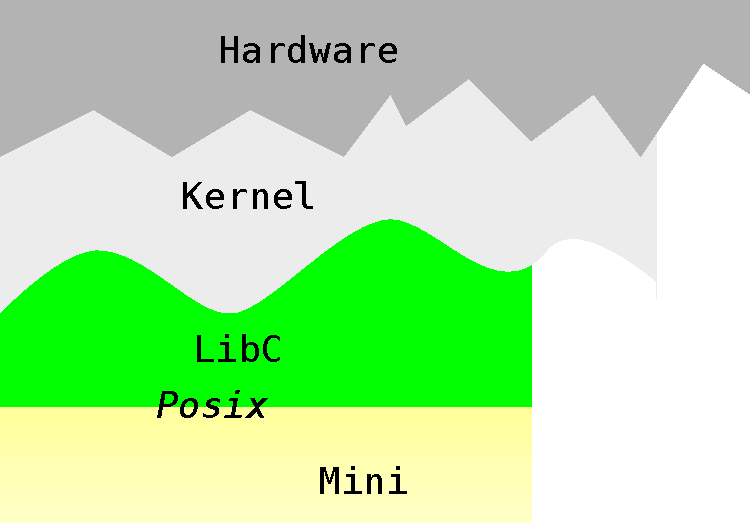
\includegraphics[width=0.75\textwidth]{mini.pdf}
\end{center}
\vspace{-5mm}
\begin{itemize}
 \item \cod{config/Makefile}
 \item \cod{src/mini.c}
 \begin{itemize}
  \item static
  \item dynamic
 \end{itemize}
\end{itemize}
\end{frame}

\subsection{Libraries}

\begin{frame}{Statische/Dynamische Bibliothek}{Kopie vs. Referenz}
 \begin{columns}
  \begin{column}{5cm}
   \begin{block}{Static}
   \begin{itemize}
    \item \hfill \vspace{-3mm}\fig{static.pdf}{0.5}{0}
    \item {\Large fr�hes} Binden
   \end{itemize}
   \end{block}
  \end{column}
  \begin{column}{5cm}
   \begin{block}{Dynamic}
    \begin{itemize}
    \item\hfill \vspace{-3mm}\fig{dynamic.pdf}{0.5}{0}
    \item {\Large sp�tes} Binden
    \end{itemize}
   \end{block}
  \end{column}
 \end{columns}
 \begin{block}{}
  \fig{legend.pdf}{0.5}{0}
 \end{block}
\end{frame}


